\documentclass{article}
	\usepackage{booktabs}
	\usepackage{listings}
	\usepackage{geometry}
	\usepackage{graphicx}
	\geometry{left=1.8cm, right=1.8cm, top=1.6cm, bottom=1.6cm}
	\usepackage{xcolor}
	\usepackage{amsmath}
	\title{X0-Compiler Design Document}
	\usepackage[colorlinks, linkcolor=red]{hyperref}
	\author{Liu, Altair @ ilovehanhan1120@hotmail.com}
	\begin{document}
		\maketitle
		\section{Introduction}
		\subsection{Purpose}
		The purpose of conducting as technical proposal to describe the global designing of this project, containing basic functionality of the system, run-time designing and error detecting methods. This document is aimed to provide a schema of designing and implement all functionality, which will be the critical document during the process of developing. This document will be read by developers and testers.
		\subsection{Background}
		This project is to develop a \textbf{X0 Language Compiler}, which is a C-like language. This project is mainly for research and study purpose.
		\begin{center}
		\begin{tabular}{cc}
			\toprule
			Item & Detail\\
			\midrule
			Project Name & X0-Compiler(mini-C)\\
			Developing Platform & Ubuntu 18.04 64-bit\\
			Developing Tools & \textbf{Flex} and \textbf{Bison}\\
			Open Source or not & Yes \\
			\bottomrule 
		\end{tabular}\\
		\end{center}
		All source files can be found at: \url{http://github.com/SubjectNoi/X0-Compiler}, star and follow it, please $ \hat{ } \_ \hat{ } $ .
		\subsection{Remarks}
		Usage:
		\begin{lstlisting}[language={sh},numbers=left,numberstyle=\tiny,%frame=shadowbox,  
   rulesepcolor=\color{red!20!green!20!blue!20},  
   keywordstyle=\color{blue!70!black},  
   commentstyle=\color{blue!90!},  
   basicstyle=\ttfamily]  
 Ubuntu>$ git clone http://github.com/SubjectNoi/X0-Compiler
 Ubuntu>$ cd X0-Compiler
 Ubuntu>$ make
 Ubuntu>$ ./X0 [Your source file]
\end{lstlisting}  
		\section{Design Summarize}
		\subsection{Main purpose of the project}
		Following are main purposes of this project:
		\begin{itemize}
		\item Run correctly on target OS: Ubuntu 18.04 64-bit
		\item Compile X0 language
		\item Report compile error, including syntax and semantic error 
		\end{itemize}
		\subsection{Primary demand}
		The X0 compiler should compile these C-like language, detailed grammar definition will be showed in next section.
		\begin{lstlisting}[language={C},numbers=left,numberstyle=\tiny,%frame=shadowbox,  
   rulesepcolor=\color{red!20!green!20!blue!20},  
   keywordstyle=\color{blue!70!black},  
   commentstyle=\color{blue!90!},  
   basicstyle=\ttfamily]  
main {
	integer i, j, flag, cnt := 0;
	for (i := 2; i != 101; i++) {
		flag := 0;
		for (j := 2; j != i; j++) { 
			if (i % j == 0) {
				flag := 1;
				break;
			}
		}
		if (flag == 0) {
			write(i);
			cnt++;
		}
	}
	write("There're:");
	write(cnt);
	write("Primes.");
}
		\end{lstlisting}
		And correct result should be given. If there exists syntax or semantic error, compiler should report them.
		\subsection{Restrictions of Design}
		To complete this project, following restrictions should be watched out:
		\begin{itemize}
		\item Project will be only run on Ubuntu 18.04
		\item Both developing and testing should be finished before 2018-11-26T11:30:00.000Z
		\end{itemize}
		\subsection{Principles and Rules of Design}
		Following principles should be followed in the process of developing:
		\begin{itemize}
		\item Complete: implement as many features as possible
		\item Simple: try best to ensure low coupling between modules
		\item High Efficiency: try best to ensure the highest execution efficiency of virtual machine code.
		\end{itemize}
		When developing, following rules should be obey:
		\begin{itemize}
		\item All files should be named under following rules:
		\begin{center}
		\begin{tabular}{cc}
			\toprule
			File & Naming rule\\
			\midrule
			Yacc file & X0-Bison.y\\
			Lex file & X0-Lex.l\\
			Constructing file & Makefile\\
			Testing source & /TestingSrc/Test\textbf{XX}\_\textbf{[Testing Content]} \\
			Git ignore file & .gitignore \\
			\bottomrule 
		\end{tabular}\\
		\end{center}
		\item Git is used for version control
		\item Use \textbf{git fetch \&\& git pull}
		\item Use \textbf{git rm -r --cached .}
		\item Use \textbf{git add .}
		\item Use \textbf{git commit -am [Meaningful Comment]}
		\item Never \textbf{git push -f}
		\end{itemize}
		\section{Main Design}
		\subsection{Demand}
		In this sub-section, detailed grammar of X0 Language will be given:
		\begin{align}
		\textbf{program} \rightarrow & 'main', \lbrace, \textbf{statement\_list}, \rbrace \\
		\textbf{statement\_list} \rightarrow &
		\textbf{statement\_list}, \textbf{statement} \\ 
	  &| \textbf{statment} \\ 
	  &| \epsilon \\
		\textbf{statement} \rightarrow &
		\textbf{expression\_list} \\ 
	  &| \textbf{if\_statement} \\ 
	  &| \textbf{while\_statement} \\
	  &| \textbf{read\_statement} \\ 
	  &| \textbf{switch\_statement} \\ 
	  &| \textbf{case\_stat} \\ 
	  &| \textbf{write\_statement} \\
	  &| \textbf{compound\_statement} \\ 
	  &| \textbf{for\_statement} \\
	  &| \textbf{do\_statement} \\ 
	  &| \textbf{declaration\_list} \\
	  &| \textbf{continue\_stat} \\ 
	  &| \textbf{break\_stat} \\
	  &| \textbf{yarimasu\_stat}\\
	  &| \epsilon \\
		\textbf{declaration\_list} \rightarrow &
		\textbf{declaration\_list}, \textbf{declaration\_stat}\\ 
	  &| \textbf{declaration\_stat} \\ 
	  &| \epsilon \\
	  	\textbf{declaration\_stat} \rightarrow & 
	  	\textbf{typeenum},\textbf{identlist},';'\\
	  &|\textbf{typeenum},\textbf{identarraylist}\\
	  &|'const',\textbf{typeenum},\textbf{identlist},\textbf{SEMICOLONSTAT}\\
	  &|'const',\textbf{typeenum},\textbf{identarraylist}\\
	  \textbf{identlist} \rightarrow & 
	  \textbf{identdef} \\
	  &|\textbf{identlist}, ',', \textbf{identdef} \\
	  &|\epsilon \\
	  \textbf{identdef} \rightarrow &
	  IDENT \\
	  &|IDENT, ':=', \textbf{factor} \\
	  \end{align}
	  \begin{align}
	  \textbf{typeenum} \rightarrow &
	  'integer' \\
	  &|'string' \\
	  &|'bool'	\\
	  &|'real'\\
	  &|'char'\\
	  \textbf{identarraylist} \rightarrow &
	  \textbf{identarraydef} \\
	  &|\textbf{identarraylist},',',\textbf{identarraydef}\\
	  \textbf{identarraydef} \rightarrow &
	  IDENT, '[', \textbf{dimensionlist}, ']'\\
	  \textbf{dimensionlist} \rightarrow &
	  \textbf{dimension} \\
	  &|\textbf{dimensionlist},',',\textbf{dimension}\\
	  \textbf{dimension} \rightarrow &
	  INTEGER \\
	  \textbf{switch\_statement} \rightarrow &
	  'switch','(',\textbf{expression},')', '\lbrace', \textbf{case\_list},\textbf{default\_statement}, '\rbrace' \\
	  \textbf{case\_list} \rightarrow &
	  \textbf{case\_list},\textbf{case\_stat} \\
	  &|\textbf{case\_stat} \\
	  &|\epsilon\\
	  \textbf{case\_stat} \rightarrow &
	  'case',\textbf{expression},':',\textbf{compound\_statement}\\
	  &|\epsilon\\
	  \textbf{default\_statement} \rightarrow &
	  'default',':',\textbf{compound\_statement}\\
	  \textbf{continue\_stat} \rightarrow & 
	  'continue',';'\\
	  \textbf{break\_stat} \rightarrow & 
	  'break',';'\\
	  \textbf{if\_statement} \rightarrow &
	  'if','(',\textbf{expression},')',\textbf{compound\_statement},\textbf{else\_list}\\
	  \textbf{else\_list} \rightarrow &
	  'else',\textbf{compound\_statement}\\
	  &|\epsilon\\
	  \textbf{while\_statement} \rightarrow &
	  'while','(',\textbf{expression},')',\textbf{compound\_statement}\\
	  \textbf{write\_statement} \rightarrow &
	  'write','(',\textbf{expression},')'\\
	  \textbf{read\_statement} \rightarrow &
	  'read','(',\textbf{var},')'\\
	  \textbf{compound\_statement} \rightarrow &
	  '\lbrace', \textbf{statement\_list}, '\rbrace'\\
	  \textbf{for\_statement} \rightarrow &
	  'for','(',\textbf{expression},';',\textbf{expression},';',\textbf{expression},')',\\ &\textbf{compound\_statement}\\
	  \textbf{do\_statement} \rightarrow &
	  'do',\textbf{compound\_statement},'while','(',\textbf{expression},')',';'\\
	  \textbf{var} \rightarrow &
	  IDENT\\
	  &|IDENT, '[',\textbf{expression\_list},']'\\
	  \textbf{expression\_list} \rightarrow &
	  \textbf{expression} \\
	  &|\textbf{expression\_list}, ',', \textbf{expression}\\
	  \textbf{expression} \rightarrow &
	  \textbf{var},':=',\textbf{expression} \\
	  &|\textbf{simple\_expr}\\
	  \textbf{simple\_expr} \rightarrow &
	  \textbf{additive\_expr} \\
	  &|\textbf{additive\_expr},\textbf{OPR},\textbf{additive\_expr}\\
	  &|\textbf{additive\_expr},\textbf{SINGLEOPR}\\
	  &|\textbf{SINGLEOPR},\textbf{additive\_expr}\\
	  \textbf{SINGLEOPR} \rightarrow &
	  '++' | '--' | '!'\\
	  \textbf{OPR} \rightarrow & 
	  '=='|'!='|'<'|'<='|'>'|'>='|'\&\&'|'||'|'\wedge\wedge'|'<<'|'>>'\\
		\end{align}
		\begin{align}
		\textbf{additive\_expr} \rightarrow &
		\textbf{term} \\
		&|\textbf{additive\_expr}, \textbf{PLUSMINUS},\textbf{term}\\
		\textbf{PLUSMINUS} \rightarrow &
		'+'|'-'\\
		\textbf{term} \rightarrow &
		\textbf{factor} \\
		&| \textbf{term},\textbf{TIMESDIVIDE},\textbf{factor}\\
		\textbf{TIMESDEVIDE} \rightarrow &
		'*'|'/'|'\%'\\
		\textbf{factor} \rightarrow &
		'(',\textbf{expression},')'\\
		&|\textbf{var}\\
		&|INTEGER \\
		&|REAL \\
		&|STRING \\
		&|BOOL\\
		&|CHAR\\
		&|YAJU\\
		\textbf{yarimasu\_stat} \rightarrow &
		'yarimasune',';'\\
		\end{align}
		This language should follow this grammar, detailed development of every modules will be mentioned below. Following are keywords:\\
		\begin{center}
		\begin{tabular}{ccccc}
			\emph{bool} & \emph{break} & \emph{call} & \emph{case} & \emph{char} \\
			\emph{const} & \emph{continue} & \emph{default} & \emph{do} & \emph{else} \\
			\emph{exit} & \emph{false} & \emph{for} & \emph{integer} & \emph{if} \\
			\emph{main} & \emph{real} & \emph{repeat} & \emph{return} & \emph{string}\\
			\emph{switch} & \emph{true} & \emph{until} & \emph{while} & \emph{write}\\
			
		\end{tabular}\\
		\end{center}
		\subsection{Environment}
		This project is developed on Ubuntu 18.04 64-bit, using \textbf{make} and corresponding \textbf{Makefile} to construct. External tools needed are: \textbf{Bison}, \textbf{Flex}, \textbf{VsCode}, \textbf{git}.
		\subsection{Modules}
		This part contain main modules that is to be implemented in this compiler. Including not only basic functionality, but also some bonus functionality. Items with * are bonus modules.
		\begin{center}
		\begin{tabular}{cc}
			\toprule
			Module Name & Brief Description\\
			\midrule
			Variable store and load & Basic functionality\\
			*Constant store and load & Support constant identifiers\\
			*Multi-type supporting & Support integer, float, string, char and boolean\\
			*Implicit type converting & Convert integer to float if necessary \\
			read and write & Basic input and output, supporting multiple types\\
			Arithmetic operation & Basic arithmetic operation including +, -, *, /, \%\\
			Logic operation & Basic logic operation including ==, !=, etc. \\
			Instant number in instruction & Essential modules for multiple types supporting\\
			Expression & Complex, mixed type expression\\
			*Unary operator & Support ++, - -, !\\
			Basic condition statement & If-else statement\\
			Basic loop statement & Do-while, while statement\\
			*Advanced condition statement & Switch-case-default statement\\
			*Advanced loop statement & For statement\\
			*N-dimension array & Support theoretically unlimited dimension array\\
			*Break/Continue & Support break/continue in for, do-while, while, switch, etc.\\
			Error processing & Reporting Syntax and Semantic errors.\\
			Magic identifiers & 114514, 1919810, yarimasune, etc.\\
			\bottomrule 
		\end{tabular}\\
		\end{center}
		
		\subsection{Hardware}
			\begin{center}
			\begin{tabular}{cc}
			\toprule
			Item & Detail \\
			\midrule
			CPU & Intel Xeon E5-2699v3@2.30GHz(18C36T) \\
			Main Board & ASUS ROG Rampage V Extreme \\
			RAM & Corsair DDR4 2133@15-15-36-50 64GB \\
			GPU & Nvidia Geforce RTX 2080Ti 11GB $ \times $ 2 \\
			Hard Disk & Intel 750 NVMe SSD 1.2TB $ \times $ 2 \\
			OS & Ubuntu 18.04 LTS 64-bit \\
			\bottomrule
			\end{tabular}
			\end{center}
		\section{Details of modules developing}
		\subsection{Data Stack}
		To support multiple types, the structure of data stack is different with origin version, \textbf{All data are stored in Binary format, and specified by pointer}.
		\begin{lstlisting}[language={C},numbers=left,numberstyle=\tiny,%frame=shadowbox,  
   rulesepcolor=\color{red!20!green!20!blue!20},  
   keywordstyle=\color{blue!70!black},  
   commentstyle=\color{blue!90!},  
   basicstyle=\ttfamily]  
enum data_type {
	integer,
	real,
	single_char,
	boolean,
	str,
};

struct data_stack {
	enum data_type	t;
	byte		val[STRING_LEN]; // STRING_LEN is defined as Macro
};
		\end{lstlisting}
		When specifying the data, using pointer in .y source: \textbf{\emph{var = *([type]*)val}}.
		\subsection{Symbol Table}
		To support multiple types and array, the structure of symbol table is different with origin version, following is detailed structure:\\
		\begin{lstlisting}[language={C},numbers=left,numberstyle=\tiny,%frame=shadowbox,  
   rulesepcolor=\color{red!20!green!20!blue!20},  
   keywordstyle=\color{blue!70!black},  
   commentstyle=\color{blue!90!},  
   basicstyle=\ttfamily]  
enum object {
	constant_int,	constant_real,
	constant_bool,	constant_string,
	constant_char,
	variable_int,	variable_real,
	variable_bool,	variable_string,
	variable_char,
	constant_int_array,	variable_int_array,
	constant_real_array,	variable_real_array,
	constant_char_array,	variable_char_array,
	constant_bool_array,	variable_bool_array,
	constant_string_array,	variable_string_array,
	function,
};
		\end{lstlisting}
		Type \textbf{function} is not used in current version, may be function will be added in following release. Expect it!
		\begin{lstlisting}[language={C},numbers=left,numberstyle=\tiny,%frame=shadowbox,  
   rulesepcolor=\color{red!20!green!20!blue!20},  
   keywordstyle=\color{blue!70!black},  
   commentstyle=\color{blue!90!},  
   basicstyle=\ttfamily]  
struct symbol_table {
	char		name[ID_NAME_LEN];
	enum object	kind;
	int		addr;
	byte		val[STRING_LEN];
	int		init_or_nor;
	int		array_size;
	int		array_const_or_not;
	int		array_dim[MAX_ARR_DIM];
};
		\end{lstlisting}
		\subsection{ISA}
		This section mainly describe all technical details of the instruction set, including meaning, usage, etc. All instruction are in following format:
		\begin{center}
		\textbf{[operation]}, \textbf{[opran1]}, \textbf{[opran2]}
		\end{center} 
		\textbf{[operation]} include \textbf{lit}, \textbf{opr}, \textbf{lod}, \textbf{sto}, \textbf{cal}, \textbf{ini}, \textbf{jmp}, \textbf{jpc}, \textbf{off}. \textbf{[opran1]} specify the type of \textbf{[opran2]} in some operation, corresponding to following table:\\
		\begin{center}
			\begin{tabular}{ccc}
			\toprule
			Value of \textbf{[opran1]} & Type of \textbf{[opran2]} & Identifier in language \\
			\midrule
			2 & Integer & \textbf{integer} \\
			3 & Real number & \textbf{real} \\
			4 & C-like string & \textbf{string} \\
			5 & Bool val & \textbf{boolean}\\
			6 & Single char & \textbf{char} \\
			\bottomrule
			\end{tabular}
			\end{center}
		\subsubsection{lit}
		This instruction is used to load instant number to the top of data stack, leading to increment of stack top. This instruct support all type in this language. Usage: \\
		\begin{itemize}
		\item \textbf{lit, 2, 1919}
		\item \textbf{lit, 5, false}
		\item \textbf{lit, 4, "LvYingZheNiuBi"}
		\item \textbf{lit, 3, 114.514}
		\end{itemize}
		This instruction will be used in instant number expression, variable declaration, etc.
		\subsubsection{opr}
		\hypertarget{4.3.2}{}
		This instruction is the most used instruction in this compiler, accounting for all of arithmetic and logic operation and some other operation, listed in the table:\\
		\begin{center}
			\begin{tabular}{cc}
			\toprule
			Value of \textbf{[opran2]} & Operation \\
			\midrule
			0 & return from function, will be developed in following release\\
			1 & Negative the stack top, support only integer and real\\
			2 & Binary operator + \\
			3 & Binary operator - \\
			4 & Binary operator * \\
			5 & Binary operator / \\
			6 & Binary operator \% \\
			7 & Binary operator == \\
			8 & Binary operator != \\
			9 & Binary operator $ < $ \\
			10 & Binary operator $ <= $ \\
			11 & Binary operator $ > $ \\
			12 & Binary operator $ >= $ \\
			13 & Binary operator $ \&\& $ \\
			14 & Binary operator $ || $ \\
			15 & Binary operator $ \wedge\wedge $ \\
			16 & Unary operator ! \\
			17 & Bit wise $ \& $\\
			18 & Bit wise $ | $\\
			19 & Output the top of the stack, type specified by \textbf{[opran1]}\\
			20 & Input a value, put it on the top of the stack\\
			21 & Binary operator $ >> $ \\
			22 & Binary operator $ << $ \\
			23 & Pop an element from the stack\\
			24 & Binary operator ==, but will not pop value from the stack\\
			   & Used for switch-case\\
			\bottomrule
			\end{tabular}
			\end{center}
		\subsubsection{lod}
		Load a variable or constant from symbol table to the top of the stack.
		\subsubsection{sto}
		Store the top of the stack to an identifier.
		\subsubsection{cal}
		Calling function, currently unused.
		\subsubsection{ini}
		Initialize a space to store data. Top of the stack will increase by the opran 2 of this instruction.
		\subsubsection{jmp}
		Jump to the instruction of opran 2.
		\subsubsection{jpc}
		Jump to the instruction of opran 2 if the top of the stack is false.
		\subsubsection{off}
		This instruction is especially used for array accessing. This instruction calculate \\ $ \textbf{array.dimension[0:dim-1] * stack.value[0:opran 1 - 1] + stack.value[opran 1]} $ to be the offset of array accessing. Because all expression value will be calculated run-time, so this result can only be back patched to the instruction run-time, the next step of this instruction is back patch to \textbf{opran2} of the next \textbf{lod/sto} instruction.
		\subsection{Variable store and load}
		\begin{itemize}
		\item In parsing phase: Variable type can be determined when parsing, and should be return along with the un-terminal with their property for further code generating job.
		\item In declaration phase: When the variable is declared, it will be written into the symbol table with an address, if using $ var := [VALUE] $ to initialize the variable, the $ init\_or\_not $ in the symbol table will be set to \textbf{true}. Using \textbf{read()} or $ := $ to assign value will also set this flag. When calling a variable with \textbf{false} flag, compiler will raise an error. 
		\item In using phase: It should be noted that when accessing a variable, the stack top should increase, or fatal data error will be caused. Whether the variable is used duplicated or not will be checked in both declaration and using phase. In this phase, \textbf{lod, [type], [address]} will be used in calling, and \textbf{sto, [type], [address]} will be used in storing.
		\end{itemize}
		\subsection{Constant store and load}
		\begin{itemize}
		\item In parsing phase, compiler will check if constant is initialized, if not, compiler will raise an error: \textbf{\emph{Constant require initialization}}. Also, the type can be determined in this phase and should be return along with the un-terminal for further code generating job. 
		\item In declaration phase: It should be noted that constant will not occupy the stack when un-used, it will only occupy if is loaded by the instruction \textbf{lod, [type], [address]}. And declaration of a constant will not generate \textbf{sto, [type], [address]} since the value of constant can be determined in paring phase. 
		\item In using phase: Be careful, anything tend to change the value of constant in the symbol table will raise error including \textbf{read()}, \textbf{$ := $}, etc. 
		\end{itemize}
		\subsection{Multi-type supporting}
		\begin{itemize}
		\item To support multiple type, the value of all variables and constants are store in \textbf{byte} format, which means all data will be converted into \textbf{byte array} to store in the symbol table, stack, and when using these variables and constants, parser will convert them from \textbf{byte array} into their origin type through \textbf{opran 1}, which is generated \textbf{\emph{by the information provided by the un-terminal}}, so it's very important to maintain the type information in parsing stage.\\
		\item Since the compiler also support instant number, so the instruction should support multiple type instant number too, which means the structure of the instruction is different, to be specific, the \textbf{opran 2} is also \textbf{byte array} type to support instant number. The instruction load an instant number is \textbf{lit, [type], [value]}, the assignment of \textbf{opran 2} of this instruction is different with others, listed as following:\\
		\begin{lstlisting}[language={C},numbers=left,numberstyle=\tiny,%frame=shadowbox,  
   rulesepcolor=\color{red!20!green!20!blue!20},  
   keywordstyle=\color{blue!70!black},  
   commentstyle=\color{blue!90!},  
   basicstyle=\ttfamily]  
byte opran[];
if (inst.fct == lit) {
	memcpy((void*)(code[pc].opr), (const void*)opran, STRING_LEN);
}
else {
	memcpy((void*)(code[pc].opr), (const void*)&opran, STRING_LEN);
}
		\end{lstlisting}
		When using the opran of an instruction, it will be the same as following format besides string opran:\\
		\begin{lstlisting}[language={C},numbers=left,numberstyle=\tiny,%frame=shadowbox,  
   rulesepcolor=\color{red!20!green!20!blue!20},  
   keywordstyle=\color{blue!70!black},  
   commentstyle=\color{blue!90!},  
   basicstyle=\ttfamily]  
int 	opran_int 		= *(int*)	&code[pc].val;
float 	opran_float 		= *(float*)	&code[pc].val;
char 	opran_char 		= *(char*)	&code[pc].val;
bool 	opran_int 		= *(int*)	&code[pc].val == 1;
string 	opran_string 		= 		 code[pc].val;
		\end{lstlisting}
		\item This compiler support implicit type convert from \textbf{integer} to \textbf{real}, \textbf{integer} to \textbf{char}, etc. Mixed type arithmetic operation is also supported by adding type of every element in the data stack.
		\end{itemize}
		\subsection{read and write}
		In this compiler, all \textbf{expression} can be written to the console, but only non-constant \textbf{var} can be read from the console. When calling \textbf{write()}, \textbf{opr, [type], 19} will be generated, and when calling \textbf{read()}, \textbf{opr, [type], 20} will be generated. \textbf{[type]} can be specified by the property of \textbf{expression} and \textbf{var}.
		\subsection{Arithmetic operation}
		There are 3 categories of arithmetic operator:
		\begin{itemize}
		\item Binary operator and will pop value from the stack.
		\item Binary operator but will not pop value from the stack (only for \textbf{switch-case} statement).
		\item Unary operator.
		\end{itemize}
		All the operator will simply generate an instruction: \textbf{opr, [type], [opran]}.
		\subsection{Logic operation}
		There are 3 categories of logic operator:
		\begin{itemize}
		\item Binary operator and will pop value from the stack.
		\item Binary operator but will not pop value from the stack (only for \textbf{switch-case} statement).
		\item Unary operator.
		\end{itemize}
		All the operator will simply generate an instruction: \textbf{opr, [type], [opran]}. The relationship of value of \textbf{opran 2} with operation is in table in \hyperlink{4.3.2}{section 4.3.2}.
		\subsection{Expression}
		Expression contains 2 parts: assignment statement and arithmetic and logic statement.
		\begin{itemize}
		\item Assignment statement: when assigning value to a variable, a \textbf{sto, [type], [value]} will be generated. And the value of assignment statement is set to be zero. So, the compiler doesn't support assignment like \textbf{\emph{$ a := b := 10 $}}, which will be fixed in future release.
		\item Arithmetic and Logic statement: since there exist priority issue in arithmetic and logic operation, so, priority is set fixed in this compiler with 6 level.\\
		\begin{center}
			\begin{tabular}{ccc}
			\toprule
			Operator & Priority & Associativity\\
			\midrule
			$ () $ & 0 & N/A\\
			$ * $, $ / $, $ \% $ & 1 & Right-associative\\
			$ + $, $ - $ & 2 & Right-associative\\
			$ << $, $ >> $, $ | $, $ \& $ & 3 & Right-associative\\
			$ ==/\neq $, $ </\leq $, $ >/\geq $, $ \&\&/||/\wedge\wedge $ & 4 & Right-associative\\
			$ ++/-- $. $ ! $ & 5 & N/A\\ 
			\bottomrule
			\end{tabular}
		\end{center}
		\end{itemize}
		\textbf{factor} is the minimal part of an expression, it can be expression surrounded by a pair of $ () $, a variable or a constant, or just instant value, in these situations, different IR will be generated:\\
		\begin{center}
			\begin{tabular}{cc}
			\toprule
			Situation & IR \\
			\midrule
			\textbf{(expressiopn)} & Parse \textbf{expression} recursively \\
			variable & \textbf{lod, [type], [address\_data\_stack]}\\
			constant & \textbf{lit, [type], [value\_in\_symbol\_table]}\\
			Instant value & \textbf{lit, [type], [value\_parsed\_by\_lex]}\\
			\bottomrule
			\end{tabular}
		\end{center}
		After having generated the code of \textbf{factor}, the code of all operation can be generated simply in \textbf{term} and \textbf{additive\_expr} as \textbf{opr, [type], [opran]}.
		\subsection{Unary operator}
		There are 2 solution to solve unary operator, one is to design specific instruction for $ ++/-- $, however, I used following method for $ variable++/-- $, $ ++/--variable $ is similar:\\
		\begin{itemize}
		\item Since when calling $ ++/-- $, variable is called first, so the top of the stack has already contained a copy of variable.
		\item Load one more copy to the top of the stack by using \textbf{lod, [type], [address\_data\_stack]}.
		\item Load instant number 1 to the top of the stack by using \textbf{lod, 2, 1}.
		\item Do the operation by using \textbf{opr, 2, $ +/- $}
		\item Store new value to the address of the variable by using \textbf{sto, [type], [address\_data\_stack]}.
		\end{itemize}
		\centerline{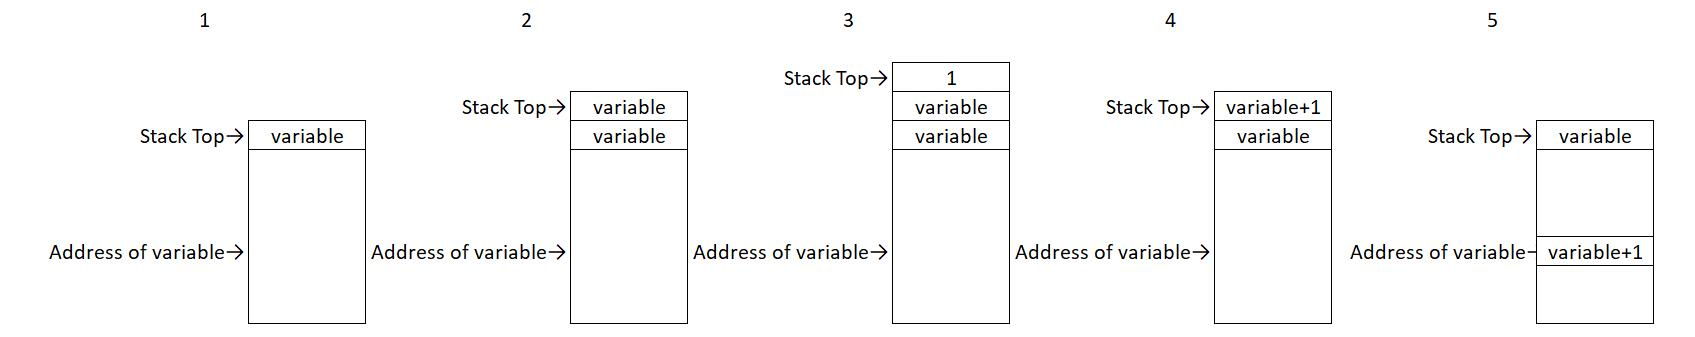
\includegraphics[width=16cm, height=3.2cm]{Pic/Pic0.jpg}}
		\subsection{Basic condition statement}
		Basic condition statement stands for \textbf{if-else} statement. Since there may be recursive if-else, while, etc. statements in an \textbf{if-else}, so the back-patch address should be recorded by the un-terminal in the grammar rather than some global variable. Detailed level condition will be discussed in \hyperlink{4.17}{section 4.17}. For \textbf{if-else} itself, first, it will generate a \textbf{jpc, 0, [destination\_address]} since there must be one condition, if \textbf{else} exists, \textbf{else} will generate an extra \textbf{jmp, 0, [destination\_address]} to jump through the statement should not be executed. The destination address will be back patched after finishing parsing the whole \textbf{if-else} statement. To be specific, the end of \textbf{if-else} will be back patched into the destination address.
		\subsection{Basic loop statement}
		Basic loop statement stands for \textbf{do-while, while} statements. Also, complex level condition will be discussed in \hyperlink{4.17}{section 4.17}. \\
		\begin{itemize}
		\item For \textbf{while} statement, first, after the expression, parser will generate a \textbf{jpc, 0, [destination\_address]}, this destination address will be back patched with the end of whole \textbf{while} statement. Then, after parsing the main body of the \textbf{while}, parser will generate a \textbf{jmp, 0, [begin\_address \_of\_expression\_in\_while]} to start a new round of condition comparing.
		\item For \textbf{do-while}, it is very similar with \textbf{while} statement, just put the \textbf{jpc, 0, [destination\_address]} before the former \textbf{jmp} in \textbf{while} statement. And back patch it with the end of whole \textbf{do-while} statement. 
		\end{itemize}
		\subsection{Advanced condition statement}
		Advanced condition statement stands for \textbf{switch-case-default} statement. Since there will be many comparing in this statement, it will be complex to use existing binary condition operators since these operators will pop result from the stack top which means the value should be calculated again. So, I implement new binary condition operators but will not pop the value from the stack top for \textbf{switch-case-default} statement. Using these operators, parser will generate a \textbf{opr, [type], $ == $(not pop stack top)} to compare the case and a \textbf{jpc, 0, [next\_case\_address]}, to back patch the address of next case, back patch list as the property of un-terminal is implemented with following structure:\\
		\begin{itemize}
		\item Structure of back patch list as the property of un-terminal. When using it, noted that a memory space should be dispatched to it by \textbf{\emph{malloc()}}.
		\begin{lstlisting}[language={C},numbers=left,numberstyle=\tiny,%frame=shadowbox,  
   rulesepcolor=\color{red!20!green!20!blue!20},  
   keywordstyle=\color{blue!70!black},  
   commentstyle=\color{blue!90!},  
   basicstyle=\ttfamily]  
struct bp_list {
	int 	case_start;
	int 	case_end;
};
%union {
	char 	*ident;
	int 	number;
	char 	*text;
	char 	single_char;
	int 	flag;
	double 	realnumber;
	struct 	bp_list *bp;
}
%type <bp>	case_stat default_statement	
		\end{lstlisting}
		\item Since there will be \textbf{break} in it, the end of the whole \textbf{switch-case-default} should be back patched to the address of every \textbf{break} statements.
		\end{itemize}
		\subsection{Advanced loop statement}
		Advanced loop statement stands for \textbf{for ($ E1 $; $ E2 $; $ E3 $) $ S $} statement. To implement this, following position should be maintained: \textbf{start of $ E2 $, start of $ S $, start of $ E3 $, end of $ S $} by additional un-terminal in the grammar. There are following steps:\\
		\begin{itemize}
		\item After parsing the condition expression $ E2 $, a \textbf{jpc, 0, [destination\_address]} will be generate if \textbf{\emph{$ E2 \neq \epsilon $}}. And a \textbf{jmp, 0, [start\_of\_$ S $]} will be generated to find the entrance of $ S $.
		\item After parsing $ S $, the iteration variable should be modified, so, a \textbf{jmp, 0, [start\_of\_$ E3 $]} will be generated to find the entrance of $ E3 $.
		\item After modifying the iteration variable, condition should be check again, so, a \textbf{jmp, 0, [start\_of\_$ E2 $]} will be generated to check again.
		\end{itemize}
		\subsection{N-dimension array}
		It should be noted that, no matter the dimension of the array, when accessing the array, the value of the expression can only be determined run-time, so, back patching is also used for array accessing. The new instruction \textbf{off} is used in this process. In the symbol table, \emph{dimension} will be maintained for the array. When accessing the array, parser will generate a \textbf{off, [number\_of\_dimension], [base\_address]} first, base address is also recorded in the symbol table. At run time, after calculated all expression in array accessing list, \textbf{off} will calculate:
		\begin{equation}
		(\sum array.dimension[0:n-1] \times stack[top-number\_of\_dimension:top-1]) + array.dimension[n]
		\end{equation}
		This will be the offset of accessing the array, last, add this offset to the base address, and back patch this result to next \textbf{lod/sto} since next \textbf{lod/sto} must be array accessing instruction. This back patch will be done \textbf{\emph{RUN TIME}}.
		\subsection{Break/Continue}
		\hypertarget{4.17}{}
		Since there may be multiple level of \textbf{for, while, if, switch}, etc. So, level should be recorded when implement \textbf{break/continue}. Every single \textbf{break/continue} will only generate a \textbf{jmp, 0, [destination\_address]}, and this destination address will be back patched in the statement call \textbf{break/continue}.
		\begin{itemize}
		\item Generate \textbf{jmp, 0, 0} at every \textbf{break/continue}.
		\item Record the \textbf{level} and address of \textbf{break/continue} to be back patched. 
		\item After parsing \textbf{for, while, if, switch}, back patch the end of them to the address of \textbf{break/continue}.
		\end{itemize}
		Since the level is implemented, when processing $ i+1 $ level, it will follow the order which means when a new \textbf{break/continue} is encountered, former \textbf{break/continue} in former \textbf{for, while, if, switch} has already been processed, so there will not be problem of data warp. After processing the $ i+1 $ level, $ i $ level will be processed, and the address of $ i+1 $ and $ i $ is stored in different location. The whole process is like a stack.
		\subsection{Error Processing}
		\begin{itemize}
		\item This compiler can't raise multiple syntax error at one time, may be it will be implemented in late release.
		\item Multiple semantic error will be raised, including:\\
		\begin{center}
			\begin{tabular}{c}
			\toprule
			Semantic Error \\
			\midrule
			Duplicated variable defined.\\
			Constant without initialized.\\
			Undefined variable.\\
			Trying to change constant.\\
			Incompatible type.\\
			Different type between boolean operator.\\
			Operators incompatible.\\
			\vdots \\
			\bottomrule
			\end{tabular}
		\end{center}
		
		\end{itemize}
		\section{Maintaining the software}
		\subsection{Maintaining Personnel}
		This software will mainly be maintained by the developer \textbf{Liu, Altair}, he can be reached by \url{ilovehanhan1120@hotmail.com}, \url{altair.liu@sap.com}.
		\subsection{Maintenance Object}
		\begin{itemize}
		\item Developer will maintain the modules that the bugs are already known.
		\item User of this software will raise report about the bugs.
		\item Optimizing and reconstructing of the software will also be conducted if developer is in a good mood, expect it.
		\end{itemize}
		\subsection{Maintenance Type}
		\begin{itemize}
		\item Bug Fixing.
		\item Code Reconstructing.
		\end{itemize}
		\subsection{Extension and Future imagination}
		Following modules may be developed if \textbf{Liu, Altair} is in a good mood.
		\begin{itemize}
		\item UI with debugger and run-time stack.
		\item function with parameter and return value.
		\item class, struct
		\item $ \Leftarrow $ To Be Continue.
		\end{itemize}
		
		
	\end{document}